% % % % % % % % % % % % % % % % % % % % % % % % % % % % % % % % % %
\documentclass[runningheads]{llncs}

\newcommand{\project}{{\sc MetaSpy}\xspace}

% packages
\usepackage{xspace}
\usepackage{ifthen}
\usepackage{amsbsy}
\usepackage{amssymb}
\usepackage{balance}
\usepackage{booktabs}
\usepackage{graphicx}
\usepackage{multirow}
\usepackage{needspace}
\usepackage{microtype}
\usepackage{bold-extra}

% constants
\newcommand{\Title}{Domain-Specific Profiling}
\newcommand{\TitleShort}{\Title}
\newcommand{\Authors}{Alexandre Bergel$^1$, Lukas Renggli, Jorge Ressia$^2$}
\newcommand{\AuthorsShort}{A. Bergel, L. Renggli, J. Ressia}

% references
\usepackage[colorlinks]{hyperref}
\usepackage[all]{hypcap}
\setcounter{tocdepth}{2}
\hypersetup{
	colorlinks=true,
	urlcolor=black,
	linkcolor=black,
	citecolor=black,
	plainpages=false,
	bookmarksopen=true,
	pdfauthor={\Authors},
	pdftitle={\Title}}

\def\chapterautorefname{Chapter}
\def\appendixautorefname{Appendix}
\def\sectionautorefname{Section}
\def\subsectionautorefname{Section}
\def\figureautorefname{Figure}
\def\tableautorefname{Table}
\def\listingautorefname{Listing}

% source code
\usepackage{xcolor}
\usepackage{textcomp}
\usepackage{listings}
\definecolor{source}{gray}{0.9}
\lstset{
	language={},
	% characters
	tabsize=3,
	upquote=true,
	escapechar={!},
	keepspaces=true,
	breaklines=true,
	alsoletter={\#:},
	breakautoindent=true,
	columns=fullflexible,
	showstringspaces=false,
	basicstyle=\footnotesize\sffamily,
	% background
	frame=single,
    framerule=0pt,
	backgroundcolor=\color{source},
	% numbering
	numbersep=5pt,
	numberstyle=\tiny,
	numberfirstline=true,
	% captioning
	captionpos=b,
	% formatting (html)
	moredelim=[is][\textbf]{<b>}{</b>},
	moredelim=[is][\textit]{<i>}{</i>},
	moredelim=[is][\color{red}\uwave]{<u>}{</u>},
	moredelim=[is][\color{red}\sout]{<del>}{</del>},
	moredelim=[is][\color{blue}\underline]{<ins>}{</ins>}}
\newcommand{\ct}{\lstinline[backgroundcolor=\color{white},basicstyle=\footnotesize\ttfamily]}
\newcommand{\lct}[1]{{\small\tt #1}}

% tikz
% \usepackage{tikz}
% \usetikzlibrary{matrix}
% \usetikzlibrary{arrows}
% \usetikzlibrary{external}
% \usetikzlibrary{positioning}
% \usetikzlibrary{shapes.multipart}
% 
% \tikzset{
% 	every picture/.style={semithick},
% 	every text node part/.style={align=center}}

% proof-reading
\usepackage{xcolor}
\usepackage[normalem]{ulem}
\newcommand{\ra}{$\rightarrow$}
\newcommand{\ugh}[1]{\textcolor{red}{\uwave{#1}}} % please rephrase
\newcommand{\ins}[1]{\textcolor{blue}{\uline{#1}}} % please insert
\newcommand{\del}[1]{\textcolor{red}{\sout{#1}}} % please delete
\newcommand{\chg}[2]{\textcolor{red}{\sout{#1}}{\ra}\textcolor{blue}{\uline{#2}}} % please change
\newcommand{\chk}[1]{\textcolor{ForestGreen}{#1}} % changed, please check

% comments \nb{label}{color}{text}
\newboolean{showcomments}
\setboolean{showcomments}{true}
\ifthenelse{\boolean{showcomments}}
	{\newcommand{\nb}[3]{
		{\colorbox{#2}{\bfseries\sffamily\scriptsize\textcolor{white}{#1}}}
		{\textcolor{#2}{\sf\small$\blacktriangleright$\textit{#3}$\blacktriangleleft$}}}
	 \newcommand{\version}{\emph{\scriptsize$-$Id$-$}}}
	{\newcommand{\nb}[2]{}
	 \newcommand{\version}{}}
\newcommand{\rev}[2]{\nb{Reviewer #1}{red}{#2}}
\newcommand{\ab}[1]{\nb{Alexandre}{blue}{#1}}
\newcommand{\lr}[1]{\nb{Lukas}{orange}{#1}}
\newcommand{\jr}[1]{\nb{Jorge}{cyan}{#1}}

% graphics: \fig{position}{percentage-width}{filename}{caption}
\DeclareGraphicsExtensions{.png,.jpg,.pdf,.eps,.gif}
\graphicspath{{figures/}}
\newcommand{\fig}[4]{
	\begin{figure}[#1]
		\centering
		\includegraphics[width=#2\textwidth]{#3}
		\caption{\label{fig:#3}#4}
	\end{figure}}

% abbreviations
\newcommand{\ie}{\emph{i.e.,}\xspace}
\newcommand{\eg}{\emph{e.g.,}\xspace}
\newcommand{\etc}{\emph{etc.}\xspace}
\newcommand{\etal}{\emph{et al.}\xspace}

% lists
\newenvironment{bullets}[0]
	{\begin{itemize}}
	{\end{itemize}}

\newcommand{\seclabel}[1]{\label{sec:#1}}
\newcommand{\co}[1]{{\sf #1}}


% D O C U M E N T
% % % % % % % % % % % % % % % % % % % % % % % % % % % % % % % % % %
\begin{document}

% T I T L E
% % % % % % % % % % % % % % % % % % % % % % % % % % % % % % % % % %

\title{\Title}
\titlerunning{\TitleShort}

\author{\Authors} 
\authorrunning{\AuthorsShort}

\institute{$^1$ PLEIAD Lab, University of Chile, Santiago, Chile\\
	\url{http://pleiad.dcc.uchile.cl} \\[0.3cm]
	$^2$ Software Composition Group, University of Bern, Switzerland\\
	\url{http://scg.unibe.ch}\\[0.3cm]
%	\url{abergel@dcc.uchile.cl}\\
%	\url{renggli@me.com}\\
%	\url{jorge.ressia@gmail.com}
	}

\maketitle

% A B S T R A C T
% % % % % % % % % % % % % % % % % % % % % % % % % % % % % % % % % %

\begin{abstract}
	Domain-specific languages and models are increasingly used within general-purpose host languages. While traditional profiling tools perform well on host language code itself, they often fail to provide meaningful results if the developers start to \ugh{abstract from traditional source code}. In this paper we demonstrate the need of dedicated profiling tools with three different case-studies. Furthermore, we present an infrastructure that enables developers to quickly prototype new profilers for their domain-specific models or languages.
\end{abstract}

% % % % % % % % % % % % % % % % % % % % % % % % % % % % % % % % % %
\section{Introduction}\seclabel{introduction}

The advances of domain-specific language and modeling reveals a drastic change in the way software is being built. The need to better define software application domain favored metamodels to be considered as first class-entities. The software engineering community has seen a rapid emergence of domain-specific tools, ranging from tools to easily build domain-specific languages~\cite{Viss04a}, transform models~\cite{Tisi10a} and language checking and embedding tools~\cite{Reng10a}.

%Whereas domain specification and definition received a fair amount of attention from the research community, domain profiling and debugging remains largely under considered. 
Whereas research on domain-specific languages made consistent progress on language specification, implementation and verification, little has been done on profiling. \ab{We need to strengthen this paragraph with some references}

This paper is about proposing a general solution for profiling specific domains. It gives the essential properties an effective domain-specific profiler must meet. It is important to notice that, as metamodels are becoming first class entities, a profiler's measurement dimension cannot be solely limited to execution time. We consider profiling as the activity to record and analyze a program execution. Profiling is essential to analyze complex data that otherwise would be to hard to harvest and compare by normal debugging.

The properties we identified a domain-specific profiler must be designed around are \emph{identifiable domain}, \emph{recordable domain events}, \emph{presentable} and \emph{evolvable}. By fulfilling these properties, a profiler will be able to be effective at identifying anomalies and sub-optimal configuration in the way a particular domain is treated.
These properties are illustrated on 3 profilers for the domains: mondrian visualizations, Omnibrowser graph models and PetitParser grammars. These profilers were designed to assess the quality of the domain modeling. A number of bugs and issues have been identified and fixed.

As a short illustration, consider the Mondrian visualization engine\footnote{Mondrian will be detailed in the coming section (\autoref{mondrian}).}. A visualization is described in terms of nodes and edges. One of the important performance and issues we recently faced is the refresh frequency: nodes and edges were simply refreshed too often\footnote{This has triggered a large discussion on the Moose mailing list (\url{http://bit.ly/fwsRbp}).}. Standard code profilers did not help to fix this since they are just able to give the share the CPU spent in the method \co{\#displayOn:} of the class \co{MONode} and \co{MOEdge}. The problem has been solved without standard profiler by identifying \emph{which} nodes and edges were indeed refreshed too often. Knowing the presence of some particular frames on the method call stack (as the majority of code profiler gives) has not been useful. The domain, defined in terms of nodes and edges, used by Mondrian is completely ignored by standard code profiler since they can only consider classes, method and stack frame. This problem, and many more, have been successfully addressed with adequate domain-specific profilers.

The contributions of this paper are: (1) the identification of the need for domain-specific profilers, (2) the presentation of several real-world case-studies where domain-specific profilers helped to significantly improve performance and correctness of domain-specific code, and (3) the presentation of an infrastructure for prototyping domain-specific profilers.

The remainder of this paper is structured as follows: \autoref{sec:problem} illustrates the problems of using a general-purpose profiler on code building on top of domain-specific language. \autoref{sec:profiler} introduces our approach to domain-specific profiling with three case-studies. \autoref{sec:implementation} presents our infrastructure to implement domain-specific profilers; and \autoref{sec:conclusion} summarizes the paper and discusses future work.

% % % % % % % % % % % % % % % % % % % % % % % % % % % % % % % % % %
\section{Problem}\seclabel{problem}

Current application profilers are useful to gather runtime data (\eg method invocations, method coverage, call trees, memory consumption) from the static code model offered by the programming language (\eg packages, classes, methods, statements). This is an effective approach when the code model is what has to be profiled. 

However, traditional profilers can hardly be used on a domain different than the code model. In many today's software there is a significant gap between the model offered by the execution platform and the model of the actually running application. The proliferation of meta-models and domain-specific languages builds new abstractions that map to the underlying execution platform in non-trivial ways. Traditional profiling tools fail to display relevant information in the presence of such abstractions.


%:=========
\subsection{Difficulty of profiling a specific domain} \label{mondrian}

This section illustrates two shortcomings of traditional profiling techniques when applied to a specific domain.\\

\paragraph{CPU time profiling.}
Mondrian\footnote{\url{http://www.moosetechnology.org/tools/mondrian}}~\cite{Meye06a} is an open and agile visualization engine. 
Mondrian uses a graph, made of (possibly nested) nodes and edges, to describe a visualization. Mondrian is a crucial component which is used in more than a dozen independent projects. To meet clients performance requirements, Mondrian's authors are paying a great attention to provide fast and scalable rendering. In June 2010 a serious performance issue was identified\footnote{\url{http://bit.ly/g8GjIh}} when visualizing an enriched dependency structural matrix~\cite{Lava09a}. Tracking down the cause of the poor performance was not a trivial task. We first used MessageTally, the sample-based code profiled provided by Pharo\footnote{\url{http://pharo-project.org/}}.

Execution sampling approximates the time spent in an application's methods by periodically stopping a program and recording the current set of methods under executions. Such a profiling technique is relatively accurate since it has little impact on the overall execution.
Beside MessageTally, execution sampling has been adopted by almost all mainstream profilers (JProfiler\footnote{\url{http://www.ej-technologies.com}}, YourKit\footnote{\url{http://www.yourkit.com}}, xprof~\cite{Gupt92a}, hprof\footnote{\url{http://java.sun.com/developer/technicalArticles/Programming/HPROF.html}}).

MessageTally produces a textual output of in which method the interpreter spent some time when rendering the visualization. An except of the output is:

\begin{lstlisting}
54.8% {11501ms} MOCanvas>>drawOn: 
  54.8% {11501ms} MORoot(MONode)>>displayOn: 
   30.9% {6485ms} MONode>>displayOn: 
      | 18.1% {3799ms} MOEdge>>displayOn: 
     	...    
      |  8.4% {1763ms} MOEdge>>displayOn: 
      |    | 8.0% {1679ms} MOStraightLineShape>>display:on: 
      |    |  2.6% {546ms} FormCanvas>>line:to:width:color: 
    	...    
   23.4% {4911ms} MOEdge>>displayOn: 	
        ...    
\end{lstlisting}

It essentially says that the virtual machine spent about 54\% of its time in the method \ct{#displayOn:} defined in the class \ct{MORoot}. A root is the unique non-nested node that contains all the nodes of the edges of the visualization. This general profiling information says that rendering nodes and edges consumes a great share of the CPU, but it does not help pinpointing which nodes and edges are culprit of the time taken. Not all the graphical elements equally consume resources.

MessageTally considers a method call frame as the unit of the profiling information. 
Stack-based virtual machine stacks a method call frame at each message send. The large majority of execution sampling profilers center their information on such frames 
%\jr{What does this mean?}\ab{Is this better? If yes, then remove these comments}. Unfortunately, this has little benefit in explaining the cause of the experienced slowdown. 
%An \emph{ad-hoc} solution consists associating for each element the number of time it has been refreshed. 
We found out that graphical shape properties such as line width, fill color, border color were constantly computed, even though no variation in the model were produced. 
This performance issue has been solved a few days after the complain via a quantification of the \ct{#displayOn:} invocation on each objects and metric computation.
 The information collected by MessageTally was not useful to solve the problem. 

\paragraph{Coverage.} 
%\jr{rewrite, it is not clear what are we aiming here.} \ab{I worked on this section. Is this better? If yes, remove the comments}
PetitParser is a parsing framework combining ideas from scannerless parsing, parser combinators, parsing expression grammars and packrat parsers to model grammars and parsers as objects that can be reconfigured dynamically \cite{Reng10c}. %PetitParser is designed to be fast: parsing a textual input is significantly faster than SmaCC, a widely used lalr parser implemented in Pharo.

A number of grammars have been implemented, including Java, Smalltalk, XML and SQL. Grammars written in PetitParser may be large. As being the result of an engineering work, a grammar may contain unnecessary rules and duplication. Getting the coverage of a grammar for a set of referential input text is useful to identify unused and duplicated parsing rules. The \ct{if} statement parsing rule is defined as follows:

\begin{lstlisting}
PPJavaSyntaxifStatement
	^ (self tokenFor: 'if') , parExpression , statement , 
	((self tokenFor: 'else'), statement ) optional
\end{lstlisting}

This parsing rule is the combination of parsers combined with the message named comma (\ct{,}).

Beside the CPU consumption, sample-based profiling estimates the method coverage of an application: methods present in the call graph are covered by the referential input text. For example, the Java grammar\footnote{\url{http://www.squeaksource.com/PetitJava.html}} for PetitParser is defined with 210 rules. These rules are modeled with a graph a objects. Whereas MessageTally is relatively efficient in estimating the coverage of source code, it is of a little help when applied to a graph of parsers, a domain other than classes and methods.

For example, MessageTally produces a large output, in which what follows is an excerpt:

\begin{lstlisting}
          ...    
            |17.1% {34ms} PPJavaSyntaxTests(PPCompositeParserTest)>>parse:rule:
            |  17.1% {34ms} PPSequenceParser(PPParser)>>parse:
            |    17.1% {34ms} PPSequenceParser>>parseOn:
            |        ....          
            |            17.1% {34ms} PPChoiceParser>>parseOn:
            |              17.1% {34ms} PPSequenceParser>>parseOn:
            |           ....          
            |                        16.6% {33ms} PPSequenceParser>>parseOn:
            |                          14.6% {29ms} PPChoiceParser>>parseOn:
            |                            14.6% {29ms} PPSequenceParser>>parseOn:
            ...    
\end{lstlisting}

MessageTally assess the coverage of the application source code by giving the list of methods involved in an execution. Some of the methods executed when executing the \ct{PPJavaSyntaxTests} are given. However, the coverage of the application source code can hardly be related to the coverage of the considered domain, object parsers in our case.

%:=========
\subsection{Requirements for domain-specific profilers}

The two example given above are representative. They illustrate the gap between a particular domain and the source code model. We argue that to efficiently profile an arbitrary domain, the following requirements needs to be fulfilled:

\begin{itemize}
\item \emph{Specifying the domain.} Since we are concerned with what makes up a visualization in Mondrian, we are interested in the different nodes and the invocation of the \ct{displayOn:} methods, instead of focusing on the implementation classes. 

Parser objects in PetitParser are dynamically generated by applying the grammar rules on a given source text. Each parser is an instance of a subclass of \ct{Parser}. 

Being able to effectively designate the objects relevant for the profiling is essential.

\item \emph{Capturing domain related events.}
Whereas the class \ct{MOGraphElement} and its subclasses total more than 263 methods, only less than 10 methods are related to displaying and computing shape dimensions. 

 During the execution of the application, relevant changes and actions triggered by the domain have to be monitored and recorded. Monitoring too many events generates noise and distraction. 
 
\item \emph{Effectively and concisely presents the necessary information.} 
The information collected by MessageTally is textually printed, emphasizing on the method invocation. A method that invokes another will be located below it and indented. Moreover each method frame is represented has a class name and a method name, which completely ignores the identity of the object and arguments that are part of the call.

Collected information have to be presented in a fashion that the important metrics and domain object composition are on the foreground.  

%\item The evolution of the profile over time.
\end{itemize}

It is important to emphasize that the limitations we identified are not particular to MessageTally. Following MessageTally, common code profilers employ executing sampling as the way to cheaply obtain dynamic information. Unfortunately, information extracted when regularly sampling the method call stack cannot be used to profile a domain other than source code model.

% % % % % % % % % % % % % % % % % % % % % % % % % % % % % % % % % %

\section{Domain-Specific Profiler}\seclabel{profiler}

%:========
\subsection{Properties of a Domain-Specific Profiler} \label{fig:properties}

We identified four distinct properties that domain-specific profilers must fulfill to be effective:


\paragraph{Identifiable domain.}
Elements that represent a domain of interest have to be retrieved from a current execution. Elements have to be identified independently of their implementation. These elements are usually expressed in terms of objets, accessible during the application execution. 

Dealing with circularity and meta-references is a common issue when a profiler is an instance of the model being profiled. To keep the model distinct from the profiler, a scoping mechanism has to be employed~\cite{Tant10a}.


\paragraph{Recordable domain events.} Relevant events generated by the domain have to be monitored and recorded to be analyzed during or after the execution. Events are expressed in terms of the method invocation, which expose four variables: a name, an object receiver, an object emitter and a list of arguments.


\paragraph{Presentable.} Information obtained during a code execution profiling needs to be adequately presented to be exploitable. A graph (composed of nodes and edges) is a structure general enough to describe meta-models.

The profiling information need to be mapped back to the profiled model. This implies that the presentation should provide enough information to be able to navigate between the profile to the model.

%\paragraph{Homogeneous event cost.} When considering the execution time of a particular event, each event must be treated as an atomic and uniform operation, independently of the object receiver. \ab{maybe not... We need to experiment on this} \lr{I don't get it.} \lr{Maybe more ``Domain-Specific Evaluation'', \ie arguing that time-to-run, number of activations, ... does not make sense; we need domain-specific values like characters/second, refreshes/click, ...}


\paragraph{Evolvable.} Being able to see the evolution of the domain events over the time is valuable, especially when precisely analyzing the sequence of domain events is complex or not feasible. 

%:========
\subsection{The \project Framework}

\jr{We need a small explanation of this table.} 

\fig{}{1.2}{MetaSpy}{The \project framework.}


\project is a framework to easily build domain-specific profilers. 
\autoref{fig:MondrianExample} shows a simplified class diagram of \project.
There are two main abstractions: the observers and the domain-specific profilers.

An observer is responsible of adapting a domain-specific model and triggering specific actions when certain conditions are fulfilled.
These observer follow the observer pattern~\cite{Gamm95a} however there are no subscribers but the profilers.
Fulfilling the specific condition of an observer will trigger the handler defined in that observer.
Some observers work by mean of registering to already reified events. Others hook in the system by using meta-programming tricks, this is also known as instrumentation..
Installing an observer activates the registration or instrumentation and the generation of events, while uninstalling removes the instrumentation. 


Some of the observers are:
\begin{description}
	\item[Announcements.] An announcement models any type of event in a system. The announcement system is implemented as an observer pattern. This observer allows us to trigger actions when an specific announcement is signaled.
	\item[Method.] This observer provides a way of profiling when an specific method is sent to any instance of a class.
	\item[Parser.] The handler action is triggered for every reduction of the parser. \jr{this is wrong like hell, check with lukas.}
	\item[Object.] In class based object-oriented profilers it is really hard to break out of the class abstractions limitations. This observer allow us to trigger action when a single instance of a class fulfills some condition. This is called object-specific profiling.
	\item[Message Received.] This observer models when a message is received by a single instance of a class. The message name and receiver can be taken into account in the definition of the condition. 
	\item[Message Send.] This observer models when a message is sent by a single instance of a class. We can scope this instrumentation to a single or more methods.
	The message name, sender and receiver can be taken into account in the definition of the condition. 
\end{description}

Profilers are responsible for modeling the domain-specific behavior to profile the main abstractions in the each domain.
\ct{MetaSpy} class models the general behavior of any profiler. It is composed of a model which is being profiled and a list of active observer or instrumentation strategies.
Each of the different profilers are called spies. They are activated when they are installed. The installation process for each spy is defined in the \ct{setUp} method.
Each spy is responsible for its own presentation and this is modeled in the method \ct{visualize}.

We will next show specific examples of various domain-specific profilers\footnotetext{Readers unfamiliar with the syntax of Smalltalk might want to read the code examples aloud and interpret them as normal sentences: An invocation to a method named \ct{method:with:}, using two arguments looks like: \ct{receiver method: arg1 with: arg2}. The semicolon separates cascaded messages that are sent to the same receiver. For example, \ct{receiver method1: arg1; method2: arg2} sends the messages \ct{method1:} and \ct{method2:} to \ct{receiver}. Other syntactic elements of Smalltalk are: the dot to separate statements: \ct{statement1. statement2}; square brackets to denote code blocks or anonymous functions: \ct{[ statements ]}; and single quotes to delimit strings: \ct{'a string'}. The caret \ct{^} returns the result of the following expression.}.

%\begin{tabular}{c|c|c}
%					&	\textbf{Host language} 	& \textbf{DSL} \\ \hline
%					&						& 		\\
%\textbf{$M_0$ - Static}	&	classes, methods		& 		\\
%					&						& 		\\\hline
%					&						& Mondrian\\
%\textbf{$M_1$ - Dynamic}	&	method activation		& OB-metamodel\\
%					&						& Grammars\\ \hline
%					&						& OB Browser\\
%\textbf{$M_2$ -} 		&						& Visualization\\
%					&						& Mondrian
%\end{tabular}


%:========
\subsection{Case Study: Caches in Mondrian}

%\jr{Is this example related to the one in section 2? if yes how, we have to build the flow here otherwise is a bunch of separated examples.} \ab{Is this better now? If yes, remove these 2 comments}

The performance issue of Mondrian described earlier (\autoref{sec:problem}) is rooted in a complex combination of different aspects of Mondrian rendering: redundancy of metrics calculation and unnecessary graphical elements repaint. Theses two aspects were independently addressed, using a dedicated profiler.

\paragraph{Keeping track of the caches activations.}
Each node has a number of caches. Activation of theses caches are under complex rules which depends on what is currently displayed, the nesting of nodes and their size. An improper implementation of the caches is a source of hard-to-track bugs and abnormal behavior. Mondrian offer two kind of caches:
\begin{itemize}
\item A node may nest other nodes and edges. The \emph{bitmap form cache} avoid to render inner nodes by snapshooting a bitmap of the nesting node. Once the bitmap cache loaded, inner nodes are not rendered any further.
\item The shape of a graphical element is the result of metric calculation on the model object represented by the element. Each dimension of a graphical element is mapped to a metric. The \emph{metric cache} avoid having to recompute the metrics at each rendering.
\end{itemize}

Keeping track of the activation and deactivation of theses two caches is realized with a dedicated profiler, called {\sc MondrianCacheActivation}. The profiler is implemented as a class \co{MSMondrianActivationCacheSpy}. The class inherits from \co{MSAbstractMondrianSpy}, which will be used for the second profiler.

{\sc MondrianCacheActivation} is defined as follows:

\begin{lstlisting}[numbers=left]
<b>MSMetaSpy subclass: #MSAbstractMondrianSpy</b>
	instanceVariableNames: 'nodes'
	
<b>MSAbstractMondrianSpy>>setUp</b>
	super setUp.
	nodes := self model root allNodes.
	
<b>MSAbstractMondrianSpy subclass: #MSMondrianCacheActivationSpy</b>

<b>MSMondrianActivationCacheSpy>>visualizeOn: view</b>
	view interaction every: 1500 do: [
		view root clear.
		view shape rectangle
			if: #hasCachedForm fillColor: Color red.

		view nodes: nodes forEach: [:each |
			view nodes: each metricCaches.
			view gridLayout gapSize: 2.
		].  
		view edges: nodes from: #owner to: #yourself.
		view treeLayout.
		view root applyLayout ]
\end{lstlisting}

The code opens a new Mondrian visualization that visualizes the profiling the nodes of another visualization, given by an \co{nodes} instances variable. The \emph{domain} that is profiled are the node. Lines 7 and 12 describes the following steps: nodes are displayed and the ownership (nesting) is represented with edges. The domain is profiled against two relevant properties. These are represented in Lines 14 and 17: a bitmap form and metrics. The profile is presented via the Mondrian script given above. The evolution over execution is realized via a periodical refresh, indicated in the script at Line 11. The model being profiled and the profiler are represented with different objects in the host language. The scope of the profiling is naturally given by operating on a different object.

\fig{}{.8}{MondrianExample}{Profiling of a Mondrian visualization in Mondrian.}

The profile visualization is given in \autoref{fig:MondrianExample}. The upper part is a visualization example, part of Mondrian tutorial. The below part is a profile of it. Upper nodes are nesting nodes. The red color indicates that the bitmap form cache is activated, and inner nodes represent metric caches. We can see that the fourth red node does not have any metric cache activated. This helped us to fix a number of issues related to the way caches are managed. These issues have been fixed in the Version 6, 9 and 10 of the package Mondrian-Core\footnote{All Mondrian versions are available online at \url{http://www.squeaksource.com/Mondrian.html}.}.


\paragraph{Number of \co{\#displayOn:} invocation.}
A Mondrian visualization may comprise a great deal of graphical elements. At each refresh of the Mondrian visualization dictated by the operating system, only the elements that needs to be refreshed must effectively be. Elements that are outside the window or for which their nesting node has an active bitmap form cache should not be rendered. 

A graphical element is rendered when the method \co{\#display:on:} is invoked. Monitoring when these invocations occur is key to have a global view of what get refreshed. 

The \project framework is instantiated to create the {\sc MondrianDisplayOn} profiler, implemented with a class \co{\sf MSMondrianSpy}:

\begin{lstlisting}
MSAbstractMondrianSpy subclass: #MSMondrianDisplayOnSpy
	instanceVariableNames: 'actualCounter previousCounter'
\end{lstlisting}

{\sf MSMondrianSpy} defines two instance variables: {\sf actualCounter} keeps track of the actual amount of events and {\sf previousCounter} the amount of events that were recorded before a new action in the profiled Mondrian visualization. These two variables are necessary to monitor the evolution of the amount of emitted events (the \emph{Profile evolution} property, listed in \autoref{fig:properties}). Subtracting the value stored in {\sf previousCounter} from {\sf actualCounter} gives the difference from two Mondrian refreshs.

\begin{lstlisting}
MSMondrianSpy>>initialize
	super initialize.
	actualCounter := IdentityDictionary new.
	previousCounter := IdentityDictionary new
\end{lstlisting}

The installation and instrumentation of Mondrian by \project is realized by the {\sf setUp} method:

\begin{lstlisting}
MSMondrianSpy>>setUp
	self model root allNodes do: [ :node |
		self 
			observeObject: node
			selector: #displayOn:
			do: [ :receiver :selector :arguments |
				actualCounter 
					at: receiver
					put: ((actualCounter at: receiver ifAbsentPut: [ 0 ]) + 1) ] ]
\end{lstlisting}

All the nodes obtained from the root of the model object are ``observed'' by the framework. At each invocation of the {\sf \#displayOn:} method, the block given as parameter to {\sf \#do:} is executed with the object receiver on which {\sf \#displayOn:} is invoked, the selector name and the argument. This block updates the number of displays for each node of the visualization.

The profiling of Mondrian is visualized using Mondrian itself. The following \co{\#visualizeOn:} method describes the visualization given in \autoref{fig:MondrianProfiler}.

\begin{lstlisting}
MSMondrianSpy>>visualizeOn: view
	view interaction every: 250 do: [ 
	...
	view nodes: self model root allNodes forEach: [ :each |
		... ].
	view verticalLineLayout.	
	view announcer on: WindowClosed do: [:ann | self uninstall ]
\end{lstlisting}

\fig{}{.8}{MondrianProfiler}{Profiling the \emph{System Complexity} visualization.}

One important point of \co{\#visualizeOn:} is to regularly update the visualization, complying with the \emph{Profile evolution} property. The profiler is uninstalled when the profiler Mondrian visualization is closed.

\autoref{fig:MondrianProfiler} gives a screenshot of a visualization and the profiler. The right-hand side is an example of the \emph{System Complexity} visualization~\cite{Lanz03d} of the collection class hierarchy in Pharo. The left hand side shows the profiler applied to the visualization. The horizontal bar indicates the amount of times the corresponding node has been displayed. %This visualization has been obtained by dragging and dropping the \ct{Collection} node

This visualization helps identifying unnecessary render of graphical element. This problem is addressed in the version 2.30 of Mondrian\footnote{\url{http://code.google.com/p/moose-technology/issues/detail?id=450}}. 

%:========
\subsection{Case Study: Events in Omnibrowser}

OmniBrowser~\cite{Berg08c} is a framework to define and compose new browsers : graphical list-oriented tools to navigate and edit elements from an arbitrary domain. In the OmniBrowser framework, a browser is described by a domain model that specifies the domain elements that can be navigated and edited, and a metagraph that spec- ifies the navigation between these domain elements. Nodes in the metagraph describe states the browser is in, while edges express navigation possibilities between those states. The OmniBrowser framework then dynamically composes widgets such as list menus and text panes to build an interactive browser that follows the navigation described in the metagraph.

\begin{lstlisting}
MSMetaSpy subclass: #MSOmniBrowserSpy
	instanceVariableNames: 'actualCounter previousCounter'
\end{lstlisting}

\begin{lstlisting}
MSOmniBrowserSpy>>setUp
	self 
		observeAnnouncer: self model announcer
		do: [ :ann | 
			actualCounter
				at: ann class
				put: (actualCounter at: ann class ifAbsentPut: [ 0 ]) + 1 ]
\end{lstlisting}

\begin{lstlisting}
\end{lstlisting}

%\paragraph{Meta-model instantiation}:
%\begin{lstlisting}
%	model := OBSystemBrowser onClass: Object selector: #printOn:.
%	profile := OmniProfiler 
%		profile: [ window :=  model open ]
%		inPackage: 'OmniBrowser'.
%\end{lstlisting}
%
%\paragraph{Recording events}:
%\begin{lstlisting}
%	model := OBSystemBrowser onClass: Object.
%	actualCounter := Dictionary new.
%	previousCounter := Dictionary new.
%	model announcer
%		observe: OBAnnouncement
%		do: [ :ann | actualCounter at: ann class put: (actualCounter at: ann class ifAbsentPut: [ 0 ]) + 1 ].
%\end{lstlisting}


%:========
\subsection{Case Study: Parsing Framework with PetitParser}


Rigorous test suites try to ensure that each part of the grammar is covered by tests and well specified according to the respective language standards. Validating that each production of the grammar is covered by the tests is a difficult activity. As mentioned previously, the traditional tools of the host language work on a method- and statement-level and thus cannot produce meaningful results in the context of PetitParser where the grammar is modeled as a graph of objects.

With \project we can implement the grammar coverage with a few lines of code. The instrumentation happens at the level of the primitive parser objects. The method \ct{observeParser:in:} wraps the parser object with a handler block that is called for each activation of the parser.

\begin{lstlisting}[numbers=left]
<b>PetitParserSpy>>setUp</b>
	self grammar allParsers do: [ :parser |
		self observeParser: parser in: self grammar do: [
			counter at: parser put: (counter at: parser ifAbsent: [ 0 ]) + 1 ] ]
\end{lstlisting}

Line~2 iterates over all primitive parser objects in the grammar. Line~3 attaches the event handler on Line~4 to each parser in the model. The handler then counts the activations of each parser object when we run the test suite of the grammar. This provides us with the necessary information to display the grammar coverage in a visualization as seen in \autoref{fig:grammar-coverage}.

\begin{figure}[h!tb]
	\centering
	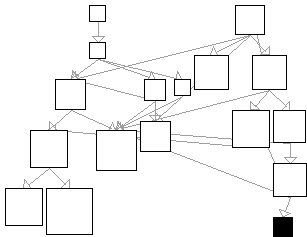
\includegraphics[width=0.4\textwidth]{xml-uncovered}
	\hspace{0.1\textwidth}
	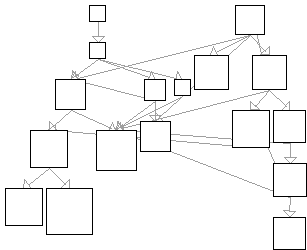
\includegraphics[width=0.4\textwidth]{xml-covered}
	\caption{Production coverage of an XML grammar with uncovered productions highlighted in black (left); and the same XML grammar with updated test coverage and complete production coverage (right). The size of the nodes is proportional to the number of activations when running the test suite on the grammar.}
	\label{fig:grammar-coverage}
\end{figure}

\ab{Which version of PetitParser correspond to the left hand side in Figure 4?} 

% % % % % % % % % % % % % % % % % % % % % % % % % % % % % % % % % %
\section{Discussion}\seclabel{discussion}

\jr{What is the objective of this section?}

\paragraph{Getting the information.} 
Depend on the application to be profiled. 
Can use events if the application to be profiled has been accordingly designed. This is the case of Omnibrowser. 

Can use bytecode instrumentation. But in that case, high level representation needs to be extracted by the programmer. A mapping has to be explicit. This is the case of PetitParser and Mondrian.




% % % % % % % % % % % % % % % % % % % % % % % % % % % % % % % % % %
\section{Implementation}\seclabel{implementation}

The implementation \project heavily relies on observers. Popularized by the Observer Design Pattern~\cite{Gamm95a}, an observer is a particular object that gets notified of any state change. The design pattern is implemented in the application to be observed. Our case is slightly different since applications can not always be prepared for an eventual profiling since a programmer cannot reliably predict which part of the software will have to be profiled in the future. This constraint significantly raises the complexity of implementing \project. 

In our situation, there are essentially two ways of implementing an observer: registering the observer with preexistent event-based systems, or using the meta-level programming techniques of the host language.

Lets consider the class \co{AnnouncementObserver}, whose responsibility is to observe the generation of specific announcements.

\begin{lstlisting}[numbers=left]
<b>AnnouncementObserver>>install</b>
	self announcer 
			on: Announcement 
			send: #value: 
			to: self handler
\end{lstlisting}

As its names says, the \co{install} method installs an observer object on the domain specified in the \co{install} method (described below). In the previous snippet of code we can see that the observer is hooked into the announcement system by evaluating the observer's handler when an announcement is triggered.

However, not all profiling activities can rely in a preexistent mechanism for registering to events. Because of this, we need to rely on the meta-programming facilities of the host language.
These facilities are not always uniform and require ad-hoc code to hook behavior in.
To avoid this drawback we decided to use a framework that provides uniform meta-programming abstractions.
Albedo~\cite{Ress10a} is a model of fined-grained unanticipated dynamic structural and behavioral adaptation. Instead of providing reflective capabilities as an external mechanism Albedo integrates them deeply in the environment. 
Albedo is a reflective system based on explicit meta-objects to improve meta-level engineering.


%Albedo~\cite{Ress10a} is a model of fined-grained unanticipated dynamic structural and behavioral adaptation. Instead of providing reflective capabilities as an external mechanism Albedo integrates them deeply in the environment. 
%Albedo is a reflective system based on explicit meta-objects, and present a series of examples illustrating how these explicit meta-objects fulfill established requirements while improving engineering at the meta-level.

Albedo's meta-objects provide a structural view and a behavioral view. In the context of \project we were mainly interested in the behavioral reifications. A behavioral meta-object reifying message send was used for the message send observer. As well as a behavioral meta-object for reifying received message. State read and write are also supported by behavioral meta-objects thus \project can profile this dynamic events.
Albedo meta-objects when attached to a single object are object-specific in nature thus fulfilling an important domain-specific profiler design requirement.

Lets consider the Message Received Observer, whose responsibility is to observe when an specific object receives an specific message.

\begin{lstlisting}[numbers=left]
<b>MessageReceivedObserver>>install</b>
	self observerMetaObject boundTo: self object
\end{lstlisting}

\begin{lstlisting}[numbers=left]
<b>MessageReceivedObserver>>setUp</b>
	profilingMetaObject := BehaviorMetaObject new 
								when: self selector 
								isReceivedDo: self handler
\end{lstlisting}
The method \ct{install} binds a meta-object to the object to be observed.
The method \ct{setUp} initializes the profiling meta-object with a behavioral meta-object. 
This meta-object evaluates the handler when a specific message is received by the profiled object. This mechanism is termed \emph{object-specific instrumentation}.

Object-specific instrumentation is not trivial to achieve in class-based languages like Smalltalk and Java \ab{without a significant overhead? AspectJ has a perObject keyword I think}. 
Classes are deeply rooted in the language interpreter or virtual machine and its performance is tweaked to rely heavily on this constructs.
Moreover, most languages provide a good level of structural reflection which deals with language structural elements like classes, method, statements, \etc
But most languages do not provide a standard mechanism to reflect on the dynamic abstraction of the language.
There are no abstractions for meta-events like a message send, a message receive, a state read, \etc.

Albedo has been designed as an evolution of partial behavioral reflection for Smalltalk, which in turn was conceived as an extension of the Reflex~\cite{Tant03a}.
\ab{is the following important? I would comment out all the remaining}Since Reflex was originally realized with Java, the Albedo approach would be achievable in a more static mainstream language like Java. 
%The reason for choosing Pharo Smalltalk for implementing Albedo is that it more naturally supports \emph{unanticipated} use of reflection at run-time and supports an AST-based reflective code model.
However, a Java solution would be more static in nature: it would not be possible to remove meta-objects completely (as code cannot be changed at run-time) and the code model would not be as closely integrated with the run-time of the language.



%:========
\subsection{Benchmark}	
	
% % % % % % % % % % % % % % % % % % % % % % % % % % % % % % % % % %
\section{Conclusion}\seclabel{conclusion}

This problem is rather well generalized. For example, profiling a virtual machine is a particularly difficult activity, since instead of providing information about bytecode and primitive executions, the virtual machine talks about functions executions\footnote{\url{http://www.mirandabanda.org/cogblog/2008/12/30/the-idee-fixe-and-the-perfected-profiler/}}.

\jr{Complete and fix}


% % % % % % % % % % % % % % % % % % % % % % % % % % % % % % % % % %
\section*{Acknowledgments}

\small We gratefully thanks ...

% bibliography
% % % % % % % % % % % % % % % % % % % % % % % % % % % % % % % % %
\bibliographystyle{splncs}
\bibliography{scg}

\end{document}